\section{结果与分析}
\label{sec:results}

\subsection{固定预算记忆保留了什么（RQ1）}
\label{sec:res_memory}
表~\ref{tab:coverage} 在验证示范的 \V{n_dec} 个决策点上比较了 16 帧预算下的各种记忆。

\textbf{均匀记忆系统性地丢失采摘。}均匀记忆只覆盖 \pct{cov_u16} 的已完成采摘，只有 \pct{cnt_u16} 的决策时刻能从记忆中数清已摘数量，连最近一次采摘也只在 \pct{last_u16} 的决策中被覆盖。它每 30 帧左右保留一帧，而一次采摘只持续十几帧，因此能否保留某次采摘几乎全凭运气，与随机记忆（\pct{cov_rand}）相当；只保留最近帧的窗口更差（\pct{cov_recent}）。

\textbf{遗忘随作业时长增长，与理论一致。}如图~\ref{fig:theory}(a)(b)，均匀记忆在前 200 帧内覆盖 \pct{cov_u_early} 的已完成采摘，超过 600 帧后降到 \pct{cov_u_late}，最近一次采摘的覆盖率也从 \pct{cov_u_early} 降到 \pct{last_u_late}。命题~\ref{prop:uniform} 在所有预算下对实测覆盖率的预测误差都不超过 \V{theory_err}（图~\ref{fig:theory}(c)），说明这一缺陷是结构性的，无法通过调参消除。按事件索引可以消除对时间的依赖：平坦事件关键帧 $k=4$ 和 $k=8$ 在所有决策时刻都覆盖最近一次采摘，$k=8$ 在 600 帧以后仍覆盖至少 \pct{cov_k8_late} 的已完成采摘。

\textbf{事件索引带来预算效率，但平坦方案的容量有限。}$k=8$ 时覆盖率达到 \pct{cov_k8}，计数可恢复率达到 \pct{cnt_k8}，而记忆帧之间间隔的中位数只从 \V{gap_u} 帧增加到 \V{gap_k8} 帧；8 帧的事件记忆（$k=4$，\pct{cov_k4_b8}）已超过 16 帧的均匀记忆，接近 32 帧的均匀记忆（\pct{cov_u32}）。不过 v1 每回合至多 5 次采摘，尚在平坦方案的容量之内；表中“倒数第三”一列已显示，$k=4$ 对第三近的采摘只剩 0.136 的覆盖率。当采摘次数超过 $k/2$ 时，平坦方案同样会遗忘（图~\ref{fig:capacity}），这正是 \hem{} 引入摘要层的原因，第~\ref{sec:res_long} 节将在长时任务上检验这一点。

\begin{table}[t]
\centering
\caption{16 帧记忆保留的信息（真实结果；v1 验证示范，两任务合计 \V{n_dec} 个决策点、\V{n_pairs} 个决策-采摘对）}
\label{tab:coverage}
\small
\begin{tabular}{lccccccc}
\toprule
记忆 & 事件覆盖 & 计数可恢复 & 最近 & 倒数第二 & 倒数第三 & 近果帧占比 & 间隔中位数\\
\midrule
均匀（K0） & 0.570 & 0.431 & 0.675 & 0.472 & 0.416 & 0.042 & 14\\
最近帧窗口 & 0.080 & 0.046 & 0.145 & 0.000 & 0.000 & 0.049 & 209\\
随机 & 0.432 & 0.329 & 0.533 & 0.351 & 0.231 & 0.040 & 41\\
平坦 $k=2$ & 0.729 & 0.579 & 1.000 & 0.430 & 0.336 & 0.085 & 17\\
\textbf{平坦 $k=4$} & \textbf{0.876} & \textbf{0.814} & \textbf{1.000} & \textbf{1.000} & 0.136 & 0.110 & 17\\
\textbf{平坦 $k=8$} & \textbf{0.996} & \textbf{0.992} & \textbf{1.000} & \textbf{1.000} & \textbf{1.000} & 0.123 & 17\\
\bottomrule
\end{tabular}
\end{table}

\begin{figure}[t]
\centering
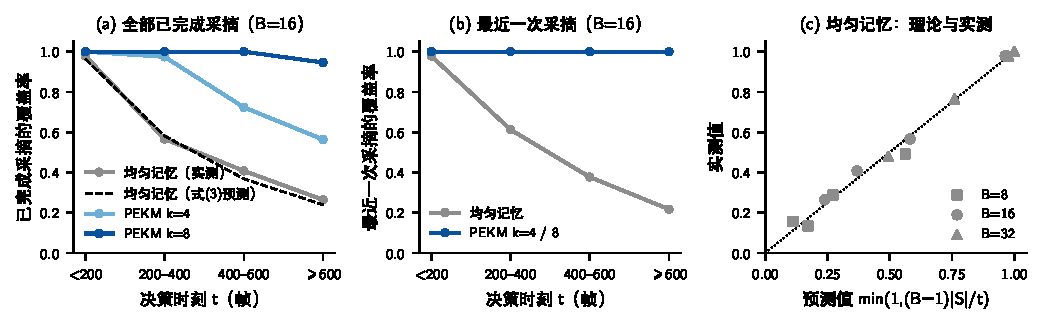
\includegraphics[width=\linewidth]{zh_coverage_theory}
\caption{按时间组织的记忆作业越久忘得越多（真实数据）。(a) $B=16$ 时全部已完成采摘的覆盖率随决策时刻的变化；(b) 最近一次采摘的覆盖率；(c) 各预算与各时间段上均匀记忆覆盖率的理论预测与实测。}
\label{fig:theory}
\end{figure}

\subsection{采摘事件检测（RQ2）}
\label{sec:res_events}
\textbf{几何事件在专家示范上精确，但在闭环中失效。}由真值距离得到的几何事件在专家示范上与真实采摘完全一致：半径在 1--4~cm 之间时，训练集和验证集上的精确率、召回率和 F1 均为 \V{evt_f1_plateau}（图~\ref{fig:events}(a)）。对距离噪声的分析给出了感知模块的精度要求：使用迟滞检测时，\V{spec_white}~cm 白噪声下 F1 为 \V{spec_white_f1}，2~cm 相关噪声下为 \V{spec_ou_f1}；而不加滤波的阈值检测在 1~cm 白噪声下 F1 即降到 \V{white1_plain_f1}，只有 \pct{white1_plain_cnt} 的回合计数正确（图~\ref{fig:events}(b)）。然而，在包含策略闭环回放的评测集上（\V{det_n_ep} 个回合，\V{det_n_ev} 次真实采摘，\V{det_n_fail} 次失败尝试），几何事件把每一次失败尝试都计为采摘，精确率降到 \V{det_geo_p}，只有 \pct{det_geo_cnt} 的回合计数正确（表~\ref{tab:detect}）。

\textbf{\pedet{} 准确、可区分成功与失败，且对光照鲁棒。}\pedet{} 的事件 F1 为 \V{det_pe_f1}，\pct{det_pe_cnt} 的回合计数正确，只有 \pct{det_pe_fp} 的失败尝试被误计为采摘；接触关键帧误差的中位数为 \V{det_pe_tc} 帧，脱离关键帧为 \V{det_pe_tr} 帧（P90 为 \V{det_pe_tr90} 帧），K8 记忆的关键帧召回率为 \V{det_pe_kf}。手工链路 \fdm{} 在标称光照下表现良好（F1 \V{det_fdm_f1}），但它依赖颜色阈值生成提示，光照扰动下 F1 降到 \V{det_fdm_light}（图~\ref{fig:events}(c)）；这与分割实验的结论一致：给定正确的提示框时 SAM 在光照变化下 F1 仍为 \V{samgt_light_f1}，失效的是颜色提示。只用夹爪开度停滞的启发式不受光照影响，但无法区分夹住果实与夹住枝叶、滑脱等情况，失败尝试误报率为 \pct{det_grip_fp}。

\textbf{两种模态互补。}只用视觉时 \pedet{} 已明显优于启发式方法（F1 \V{det_pv_f1}），但在腕部画面被果实或叶片大面积遮挡时会漏检；只用本体感知时 F1 为 \V{det_pp_f1}，对“夹住但未脱离”与“已脱离”的区分较差。两者融合后误报率降到 \pct{det_pe_fp}，说明视觉提供“夹住的是不是果实、果实是否离开果柄”，本体感知提供“夹爪何时闭合、受力如何变化”。

\begin{table}[t]
\centering
\caption{采摘事件检测（仿真 v2 验证集，含专家示范与闭环回放）}
\label{tab:detect}
\small
\setlength{\tabcolsep}{4.5pt}
\begin{tabular}{lcccccc}
\toprule
检测器 & 精确率 & 召回率 & F1 & 计数正确（\%） & 失败尝试误报（\%） & 光照扰动 F1\\
\midrule
几何事件（真值距离，特权） & \V{det_geo_p} & \V{det_geo_r} & \V{det_geo_f1} & \V{det_geo_cnt} & \V{det_geo_fp} & \V{det_geo_light}\\
\fdm{}（手工感知链路） & \V{det_fdm_p} & \V{det_fdm_r} & \V{det_fdm_f1} & \V{det_fdm_cnt} & \V{det_fdm_fp} & \V{det_fdm_light}\\
夹爪停滞启发式 & \V{det_grip_p} & \V{det_grip_r} & \V{det_grip_f1} & \V{det_grip_cnt} & \V{det_grip_fp} & \V{det_grip_light}\\
\pedet{}（仅视觉） & \V{det_pv_p} & \V{det_pv_r} & \V{det_pv_f1} & \V{det_pv_cnt} & \V{det_pv_fp} & \V{det_pv_light}\\
\pedet{}（仅本体） & \V{det_pp_p} & \V{det_pp_r} & \V{det_pp_f1} & \V{det_pp_cnt} & \V{det_pp_fp} & \V{det_pp_light}\\
\textbf{\pedet{}（完整）} & \textbf{\V{det_pe_p}} & \textbf{\V{det_pe_r}} & \textbf{\V{det_pe_f1}} & \textbf{\V{det_pe_cnt}} & \textbf{\V{det_pe_fp}} & \textbf{\V{det_pe_light}}\\
\bottomrule
\end{tabular}
\end{table}

\begin{figure}[t]
\centering
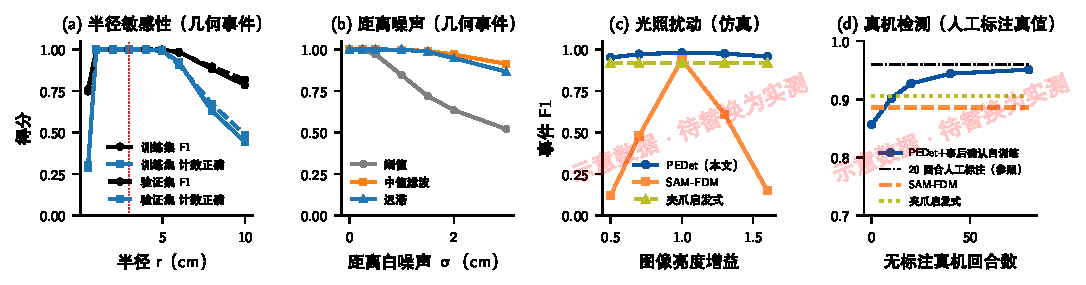
\includegraphics[width=\linewidth]{zh_event_detection}
\caption{事件检测。(a) 几何事件的 F1 与计数正确率随半径 $r$ 的变化（真实）；(b) 几何事件在距离白噪声下的 F1，比较阈值、中值滤波与迟滞三种检测（真实）；(c) 图像亮度增益扰动下三种检测器的事件 F1；(d) 真机上事件 F1 随无标注回合数的变化（事后确认自训练），真值为第三视角人工标注，点划线为 20 个人工标注回合的有监督参照。}
\label{fig:events}
\end{figure}

\subsection{仿真闭环主结果（RQ3）}
\label{sec:res_closed}
\textbf{正对照确认任务都在检验记忆。}在推理时只给 K0 保留最近 16 帧，计数 v2 的记忆类失败率从 \pct{pc_cnt_a} 升到 \pct{pc_cnt_b}（\V{pc_cnt_d}~\pp，95\% CI \V{pc_cnt_ci}），遮挡 v2 从 \pct{pc_occ_a} 升到 \pct{pc_occ_b}（\V{pc_occ_d}~\pp，CI \V{pc_occ_ci}），均远超预设的 15~\pp{} 门槛。与 v1 不同，v2 任务的成败确实取决于长程记忆。

\textbf{HarvestMem 大幅提高了事件记忆任务的成功率。}表~\ref{tab:closed} 与图~\ref{fig:simmain}(a) 给出主结果。在计数 v2 上，K0 的成功率为 \pct{c_k0_s}，HEM 达到 \pct{c_hem_s}，提高 \V{c_dh}~\pp（95\% CI \V{c_dh_ci}，Holm $p$ \V{c_dh_p}），主假设 H1 获得支持；平均计数误差 $|\text{入篮数}-N|$ 从 \V{c_k0_err} 颗降到 \V{c_hem_err} 颗。平坦关键帧同样有效（K4 \V{c_d4}~\pp，K8 \V{c_d8}~\pp），说明“按事件组织记忆”本身是增益的主要来源；HEM 相对 K8 再提高 \V{c_dh8}~\pp（CI \V{c_dh8_ci}），差距较小，与事先预测一致：计数 v2 的配额 $N\le5$ 基本在 K8 的容量之内。关闭安全包络后，HEM$-$K0 为 \V{c_dh_noguard}~\pp（CI \V{c_dh_noguard_ci}），结论不依赖包络；各条件的包络裁剪率接近（约 \pct{c_clip}）。

\textbf{场景记忆任务上各条件等效，与事先预测一致。}在遮挡 v2 上，K0、K4、K8 与 HEM 的成功率分别为 \pct{o_k0_s}、\pct{o_k4_s}、\pct{o_k8_s} 和 \pct{o_hem_s}；HEM$-$K0 为 \V{o_dh}~\pp（CI \V{o_dh_ci}），TOST 检验在 $\pm10$~\pp{} 等效界内成立（$p=\V{o_dh_tost}$）。这一“预测中的无差异”同样重要：它表明 HarvestMem 的增益只出现在信息以事件形式存在的场合，而为事件分配位置并没有挤掉阵风前的关键画面，因为场景锚层始终保留第 0 帧。

\textbf{增益随配额增大，且越接近平坦方案的容量上限，分层的优势越明显。}如图~\ref{fig:simmain}，HEM 相对 K0 的增益在 $N=2$、3、4--5 时分别为 \V{cN_gain_h0.1}、\V{cN_gain_h0.2} 和 \V{cN_gain_h0.3}~\pp；相对 K8 的增益分别为 \V{cN_gain_h8.1}、\V{cN_gain_h8.2} 和 \V{cN_gain_h8.3}~\pp，在 $N=5$ 超过 K8 的 4 次容量时开始显现。配额越大，回合越长、事件越多，均匀记忆按命题~\ref{prop:uniform} 丢失得越多。

\begin{table}[t]
\centering
\caption{仿真闭环结果（val 150--199 $\times$ 种子 7/8/9，每格 \V{n_val} 次；差值单位为百分点，方括号为 95\% CI）}
\label{tab:closed}
\small
\setlength{\tabcolsep}{2.6pt}
\begin{tabular}{llcccccc}
\toprule
任务 & 记忆 & \shortstack{成功率\\（\%）} & \shortstack{记忆类\\失败（\%）} & \shortstack{操作类\\失败（\%）} & \shortstack{计数误差\\（颗）} & $\Delta$ vs K0 & $\Delta$ vs K8\\
\midrule
\multirow{4}{*}{\shortstack{计数 v2\\（事件记忆）}} & K0 均匀 & \V{c_k0_s} & \V{c_k0_mem} & \V{c_k0_op} & \V{c_k0_err} & -- & --\\
 & K4 平坦 & \V{c_k4_s} & \V{c_k4_mem} & \V{c_k4_op} & \V{c_k4_err} & \V{c_d4} \V{c_d4_ci} & --\\
 & K8 平坦 & \V{c_k8_s} & \V{c_k8_mem} & \V{c_k8_op} & \V{c_k8_err} & \V{c_d8} \V{c_d8_ci} & --\\
 & \textbf{HEM} & \textbf{\V{c_hem_s}} & \textbf{\V{c_hem_mem}} & \V{c_hem_op} & \textbf{\V{c_hem_err}} & \textbf{\V{c_dh}} \V{c_dh_ci}\textsuperscript{H1} & \V{c_dh8} \V{c_dh8_ci}\\
\midrule
\multirow{4}{*}{\shortstack{遮挡 v2\\（场景记忆）}} & K0 均匀 & \V{o_k0_s} & \V{o_k0_mem} & -- & -- & -- & --\\
 & K4 平坦 & \V{o_k4_s} & \V{o_k4_mem} & -- & -- & \V{o_d4} \V{o_d4_ci} & --\\
 & K8 平坦 & \V{o_k8_s} & \V{o_k8_mem} & -- & -- & \V{o_d8} \V{o_d8_ci} & --\\
 & HEM & \V{o_hem_s} & \V{o_hem_mem} & -- & -- & \V{o_dh} \V{o_dh_ci}\textsuperscript{T} & --\\
\midrule
\multirow{3}{*}{\shortstack{FruitRow\\（长时事件）}} & K0 均匀 & \V{l_k0_s} & \V{l_k0_mem} & \V{l_k0_op} & \V{l_err_k0} & -- & --\\
 & K8 平坦 & \V{l_k8_s} & \V{l_k8_mem} & \V{l_k8_op} & \V{l_err_k8} & -- & --\\
 & \textbf{HEM} & \textbf{\V{l_hem_s}} & \textbf{\V{l_hem_mem}} & \V{l_hem_op} & \textbf{\V{l_err_hem}} & \textbf{\V{l_dh0}} \V{l_dh0_ci}\textsuperscript{H2} & \textbf{\V{l_dh8}} \V{l_dh8_ci}\textsuperscript{H3}\\
\bottomrule
\end{tabular}

\vspace{2pt}
{\footnotesize H1--H3：预登记主假设，Holm 校正后 $p$ 均 \V{l_p}。T：TOST 等效检验 $p=\V{o_dh_tost}$（$\pm10$~\pp）。}
\end{table}

\begin{figure}[t]
\centering
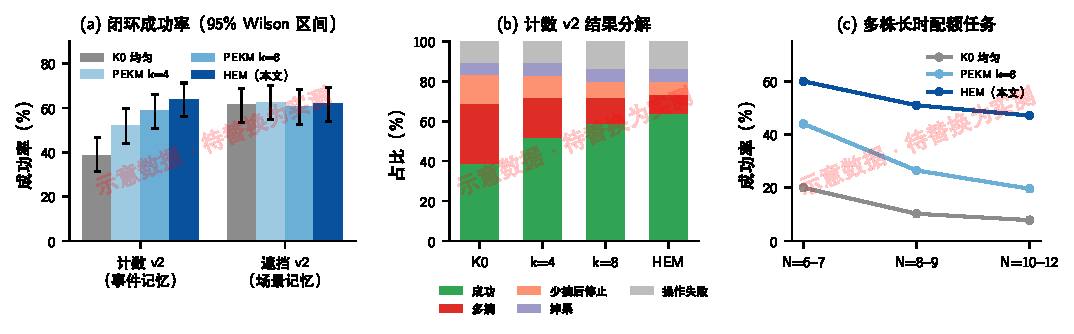
\includegraphics[width=\linewidth]{zh_sim_main}
\caption{仿真闭环结果。(a) 计数 v2 与遮挡 v2 上四种记忆的成功率；(b) 计数 v2 的结果分解，增益几乎全部来自多摘和少摘后停止这两类记忆失败的减少；(c) FruitRow 按配额 $N$ 分层的成功率，平坦关键帧在采摘次数超出其容量后迅速下降。}
\label{fig:simmain}
\end{figure}

\subsection{长时作业中的可扩展性（RQ4）}
\label{sec:res_long}
\textbf{分层记忆在长时作业中优势最大。}FruitRow 平均每回合 \V{row_events} 次采摘，远超平坦关键帧的容量。如表~\ref{tab:closed}，K0 的成功率只有 \pct{l_k0_s}，K8 为 \pct{l_k8_s}，HEM 达到 \pct{l_hem_s}：相对 K0 提高 \V{l_dh0}~\pp（CI \V{l_dh0_ci}），相对 K8 提高 \V{l_dh8}~\pp（CI \V{l_dh8_ci}），主假设 H2、H3 均获支持（Holm $p$ \V{l_p}）。平均计数误差从 K0 的 \V{l_err_k0} 颗、K8 的 \V{l_err_k8} 颗降到 \V{l_err_hem} 颗。

\textbf{性能随配额的变化与容量分析吻合。}如图~\ref{fig:simmain}(c)，当 $N$ 从 6--7 增加到 10--12，K8 的成功率从 \pct{lN_k8.1} 降到 \pct{lN_k8.3}，与它约 4 次的容量一致：更早的采摘只能依靠时间上下文层碰运气。HEM 只从 \pct{lN_hem.1} 缓降到 \pct{lN_hem.3}，下降主要来自回合变长后操作失败的累积，而不是记忆失败。这是命题~\ref{prop:capacity} 在闭环中的直接体现。

\textbf{分层结构的每个部分都必要。}表~\ref{tab:ablation}(b) 在 FruitRow 上逐一去除 \hem{} 的组件。去掉情景摘要层后，\hem{} 只保留最近 2 次采摘，成功率降到 \pct{al_nosum}，低于 K8；摘要层用单帧代替拼图（容量 5 次）时为 \pct{al_single}；改用 $3\times3$ 拼图虽把容量提高到 29 次，但每格分辨率降低、且本任务的采摘次数已在 $2\times2$ 拼图的容量之内，成功率为 \pct{al_mosaic9}，略低于默认设置。去掉类型-时间嵌入后成功率降到 \pct{al_noemb}：策略无法区分拼图帧与普通帧，也无法判断事件的先后。去掉事件扰动训练后为 \pct{al_noept}。

\subsection{增益从何而来：机制与消融（RQ5）}
\label{sec:res_ablation}
\textbf{增益来自记忆类失败的减少。}如图~\ref{fig:simmain}(b)，从 K0 到 HEM，计数 v2 的记忆类失败率从 \pct{c_k0_mem} 降到 \pct{c_hem_mem}，而操作类失败率基本不变（\pct{c_k0_op} 与 \pct{c_hem_op}）。增益集中在“多摘”上，这正是记住自己每次放果所能避免的错误。

\textbf{反事实对照排除了“换帧扰动”的解释。}表~\ref{tab:ablation}(a) 中，若保留同样数量的事件位置，但把关键帧整体错后 24 帧（不再对准接触与脱离），成功率降到 \pct{ab_shift}；若事件位置随机选取，则为 \pct{ab_random}，均与 K0 相当。改变记忆的\emph{内容}而非\emph{位置数量}才带来增益。只保留接触帧时成功率为 \pct{ab_contact}，只保留脱离帧时为 \pct{ab_release}：脱离帧显示“果实已离开果柄、正被带走”，直接对应“又摘了一颗”。

\textbf{学习型检测接近物理真值，且优于特权几何信号。}使用仿真物理事件（上界）时成功率为 \pct{ab_oracle}，\pedet{} 为 \pct{ab_pedet}，仅差 \V{ab_gap}~\pp；使用真值距离的几何事件反而降到 \pct{ab_geo}，因为闭环中的失败尝试被当作采摘写入记忆；\fdm{} 和夹爪启发式分别为 \pct{ab_fdm} 和 \pct{ab_grip}。光照扰动下，HEM+\pedet{} 保持在 \pct{ab_light_pedet}，HEM+\fdm{} 降到 \pct{ab_light_fdm}，与同样条件下的 K0（\pct{ab_light_k0}）相差无几：事件丢失时 \hem{} 自动退化为均匀记忆，而不会比均匀记忆更差。

\textbf{事件扰动训练使策略对检测误差鲁棒。}去掉 EPT 重新训练后，计数 v2 成功率从 \pct{ab_pedet} 降到 \pct{ab_noept}。在推理时人为注入 10\% 漏检，有 EPT 的策略为 \pct{ab_noise_ept}，几乎不受影响；无 EPT 的策略降到 \pct{ab_noise_noept}，多摘明显增加，说明未经扰动训练的策略会无条件信任记忆。直接在推理时给 K0 策略换上 \hem{} 记忆（训练中从未见过），成功率为 \pct{ab_untrained}，不优于 K0：训练与部署必须使用同一记忆构造函数。

\begin{table}[t]
\centering
\caption{消融与反事实对照（每项 150 次）}
\label{tab:ablation}
\small
\begin{tabular}{llc}
\toprule
因素 & 设置 & 成功率（\%）\\
\midrule
\multicolumn{3}{l}{\textbf{(a) 计数 v2，HEM 策略}}\\
默认 & HEM + \pedet{} + EPT & \textbf{\V{ab_pedet}}\\
\multirow{4}{*}{事件来源} & 仿真物理事件（上界） & \V{ab_oracle}\\
 & 几何事件（真值距离，特权） & \V{ab_geo}\\
 & \fdm{} & \V{ab_fdm}\\
 & 夹爪停滞启发式 & \V{ab_grip}\\
\multirow{3}{*}{光照扰动} & K0 均匀 & \V{ab_light_k0}\\
 & HEM + \fdm{} & \V{ab_light_fdm}\\
 & HEM + \pedet{} & \V{ab_light_pedet}\\
\multirow{2}{*}{反事实} & 关键帧错后 24 帧（位置数相同） & \V{ab_shift}\\
 & 事件位置随机选取 & \V{ab_random}\\
\multirow{2}{*}{关键帧组成} & 只保留接触帧 & \V{ab_contact}\\
 & 只保留脱离帧 & \V{ab_release}\\
\multirow{3}{*}{鲁棒训练} & 去掉 EPT（重新训练） & \V{ab_noept}\\
 & 注入 10\% 漏检：有 EPT / 无 EPT & \V{ab_noise_ept} / \V{ab_noise_noept}\\
 & K0 策略推理时改用 \hem{}（训练未见） & \V{ab_untrained}\\
\midrule
\multicolumn{3}{l}{\textbf{(b) FruitRow，HEM 结构（均重新训练）}}\\
默认 & 完整 \hem{}（$2\times2$ 拼图，容量 \V{cap_hem}） & \textbf{\V{al_full}}\\
\multirow{5}{*}{结构} & 去掉情景摘要层（容量 2） & \V{al_nosum}\\
 & 摘要层用单帧代替拼图（容量 5） & \V{al_single}\\
 & $3\times3$ 拼图（容量 29，单格分辨率更低） & \V{al_mosaic9}\\
 & 去掉类型-时间嵌入 & \V{al_noemb}\\
 & 去掉事件扰动训练 & \V{al_noept}\\
\bottomrule
\end{tabular}
\end{table}

\subsection{真实番茄采摘实验（RQ6）}
\label{sec:res_real}
\textbf{事后确认自训练无需人工标注即可完成检测器迁移。}在 \V{rb_det_ep} 个独立真机回合（\V{rb_det_ev} 次真实采摘）上，以第三视角人工标注为真值（表~\ref{tab:realdet}），仅在仿真中训练的 \pedet{} 的 F1 为 \V{rd_zero.3}，低于夹爪启发式（\V{rd_grip.3}），主要误差来自真实番茄的颜色与反光差异。经过 \V{rb_hsl_ep} 个无标注回合的事后确认自训练，F1 提高到 \V{rd_hsl.3}，与用 \V{rb_sup_ep} 个人工标注回合有监督微调的参照（\V{rd_sup.3}）几乎相当，脱离关键帧误差中位数为 \V{rd_tr} 帧。\pct{hsl_keep} 的持物段通过一致性筛选，伪标签的事件精确率为 \V{hsl_prec}。图~\ref{fig:events}(d) 显示，10 个无标注回合就足以超过两种基线。\fdm{} 在真机上受果皮反光造成的深度空洞和光照影响，F1 为 \V{rd_fdm.3}。

\textbf{真机闭环结果与仿真一致。}如图~\ref{fig:real} 与表~\ref{tab:real}，在真机计数任务上，HEM 的成功率为 \pct{rc_hem_s}，K0 为 \pct{rc_k0_s}（\V{rc_d}~\pp，配对符号翻转检验 $p=\V{rc_p}$），平均计数误差从 \V{rc_err_k0} 颗降到 \V{rc_err_hem} 颗；增益主要来自多摘的减少（K0 \V{rc_k0.2} 次，HEM \V{rc_hem.2} 次）。HEM 相对 K8（\pct{rc_k8_s}）高 \V{rc_d8}~\pp（$p=\V{rc_p8}$），真机配额 $N\le3$ 在 K8 容量之内，这一差距与仿真中计数 v2 的结果一致。在真机遮挡任务上，K0 与 HEM 分别为 \pct{ro_k0_s} 和 \pct{ro_hem_s}，符合“场景记忆无差异”的预测。在暖色光照扰动下，HEM+\pedet{} 的计数任务成功率为 \pct{rl_pedet_s}，HEM+\fdm{} 降到 \pct{rl_fdm_s}。在日光温室的盆栽番茄上，HEM 完成 \V{gh_hem} 次、K0 完成 \V{gh_k0} 次。单回合平均用时 K0 为 \V{rt_k0}~s，HEM 为 \V{rt_hem}~s，两者相当。

\begin{table}[t]
\centering
\caption{真机结果。上：采摘事件检测（\V{rb_det_ep} 回合，第三视角人工标注真值）；下：闭环结果（每条件 \V{rb_trials} 次）}
\label{tab:realdet}
\label{tab:real}
\small
\begin{tabular}{lccc}
\toprule
检测器 & 精确率 & 召回率 & F1\\
\midrule
夹爪停滞启发式 & \V{rd_grip.1} & \V{rd_grip.2} & \V{rd_grip.3}\\
\fdm{} & \V{rd_fdm.1} & \V{rd_fdm.2} & \V{rd_fdm.3}\\
\pedet{}（仅仿真训练） & \V{rd_zero.1} & \V{rd_zero.2} & \V{rd_zero.3}\\
\textbf{\pedet{} + 事后确认自训练（零标注）} & \textbf{\V{rd_hsl.1}} & \textbf{\V{rd_hsl.2}} & \textbf{\V{rd_hsl.3}}\\
\pedet{} + \V{rb_sup_ep} 回合人工标注（参照） & \V{rd_sup.1} & \V{rd_sup.2} & \V{rd_sup.3}\\
\midrule
闭环条件 & 成功率（\%） & 多摘 / 少摘停止 & 掉果 / 操作失败\\
\midrule
真机计数：K0 均匀 & \V{rc_k0_s} & \V{rc_k0.2} / \V{rc_k0.3} & \V{rc_k0.4} / \V{rc_k0.5}\\
真机计数：K8 平坦 & \V{rc_k8_s} & \V{rc_k8.2} / \V{rc_k8.3} & \V{rc_k8.4} / \V{rc_k8.5}\\
真机计数：\textbf{HEM} & \textbf{\V{rc_hem_s}} & \V{rc_hem.2} / \V{rc_hem.3} & \V{rc_hem.4} / \V{rc_hem.5}\\
真机遮挡：K0 / HEM & \V{ro_k0_s} / \V{ro_hem_s} & -- & --\\
暖光计数：HEM+\fdm{} / HEM+\pedet{} & \V{rl_fdm_s} / \V{rl_pedet_s} & -- & --\\
温室番茄：K0 / HEM（成功次数） & \V{gh_k0} / \V{gh_hem} & -- & --\\
\bottomrule
\end{tabular}
\end{table}

\begin{figure}[t]
\centering
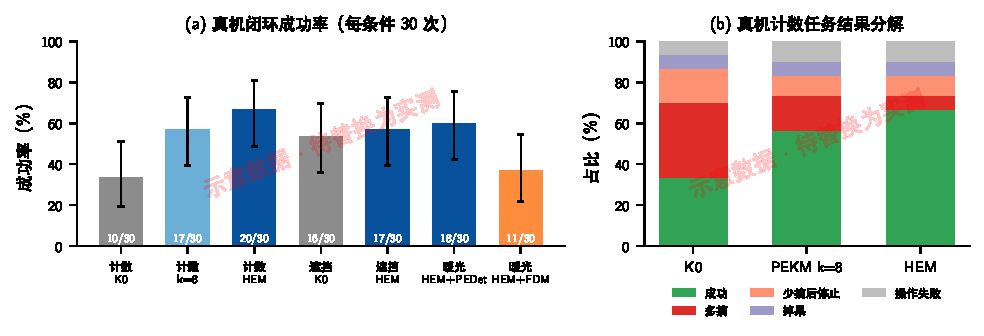
\includegraphics[width=0.92\linewidth]{zh_real}
\caption{真机闭环结果。(a) 各条件成功率与 Wilson 95\% 区间；(b) 真机计数任务的结果分解。}
\label{fig:real}
\end{figure}

\subsection{记忆内容对 VLA 策略的影响（补充证据）}
\label{sec:res_general}
本文的前提是：固定预算记忆的\emph{内容}会影响 VLA 策略的行为。我们在一个通用操作记忆基准上，以相同结构的基础策略、在封存协议和配对检验下验证了这一点（真实结果）：去掉历史记忆后，模式回忆任务成功率从 \pct{robomme_nomem_a} 降到 \pct{robomme_nomem_b}（$-65.0$~\pp，95\% CI $[-81.7,-46.7]$，$p<0.001$）；记忆预算从 32 帧减半到 16 帧，成功率从 \pct{robomme_half_a} 降到 \pct{robomme_half_b}（$-37.8$~\pp，$p<0.001$）；替换单个记忆位置会改变动作损失，位置重要性排序的可靠度在四个任务上为 0.97--0.99。也就是说，在固定预算内记住什么确实重要，而这正是 HarvestMem 利用采摘的物理结构所做的决定。

\subsection{运行开销}
\label{sec:res_cost}
表~\ref{tab:cost} 汇总了各组件的开销。\hem{} 构造一次记忆耗时约 \V{hem_ms}~ms，拼图帧只在有事件进入摘要层时编码一次；由于记忆图像数和 token 数不变，策略的显存与推理开销与均匀记忆完全相同，新增参数仅约 \V{hem_params}~M。\pedet{} 每帧耗时 \V{pedet_ms}~ms，可与控制循环并行运行。作为对比，\fdm{} 需在每回合开始时运行一次 SAM（ViT-B \V{sam_ms_b}~ms，ViT-H \V{sam_ms_h}~ms），并依赖深度相机与精确外参。

\begin{table}[t]
\centering
\caption{运行开销（仿真：NVIDIA L20；真机：\V{rb_gpu}）}
\label{tab:cost}
\small
\begin{tabular}{lll}
\toprule
组件 & 开销 & 频率\\
\midrule
均匀采样 / 平坦关键帧选帧（$t=1000$） & \V{unif_us} / \V{pekm_us}~$\mu$s（CPU 单核） & 每次决策\\
\hem{} 记忆构造（含拼图） & \V{hem_ms}~ms（CPU） & 每次决策\\
类型-时间嵌入 & 新增约 \V{hem_params}~M 参数，计算可忽略 & 每次决策\\
\pedet{} & 仿真 \V{pedet_ms}~ms；真机 \V{rt_pedet}~ms & 每控制步\\
VLA 推理（一个动作块） & 仿真 \V{sim_vla_ms}~ms；真机 \V{rt_vla}~ms & 每 16 步\\
\fdm{} 的 SAM 分割 & ViT-B \V{sam_ms_b}~ms；ViT-H \V{sam_ms_h}~ms & 每回合一次\\
\bottomrule
\end{tabular}
\end{table}
